\section{Codegenerierung}
\label{sec:codegeneration}
In bestimmten Fällen ist es mittlerweile nicht mehr notwendig Quellcode von Hand zu schreiben. Stattdessen kann spezifiziert werden, was der Programmcode tun soll und aus dieser Information automatisch Code generiert werden. Dieser Anwendungsfall kann zwar nicht so weitläufig eingesetzt werden wie die Codevervollständigung, spart stellenweise aber noch mehr Arbeit ein.

\subsection{Allgemeine Konzepte}
\label{subsec:generation_concepts}
Programmiersprachen dienen dazu Datenstrukturen und Algorithmen formal aber vom Menschen lesbar auszudrücken. Hierbei unterscheidet man zwischen High-Level- und Low-Level Programmiersprachen (\autoref{fig:abstractionLevels}). Low-Level Programmiersprachen befinden sich auf einer niedrigen, High-Level Programmiersprachen auf einer höheren Abstraktionsebene. Ziel dieser Abstraktion ist es, die Lesbarkeit zu erhöhen und die Komplexität zu reduzieren. Hierfür bieten High-Level Programmiersprachen beispielsweise Kontrollstrukturen und Datentypen an.
Bei der Codegenerierung wird diese Idee aufgegriffen und erweitert.
Im Allgemeinen geht es um die Frage, ob es nicht einfachere und kompaktere Darstellungsweisen für Problemlösungen gibt, die anschließend in Programmcode einer tieferen Abstraktionsebene umgewandelt werden können. 
\begin{figure}[!htb] 
	\centering
	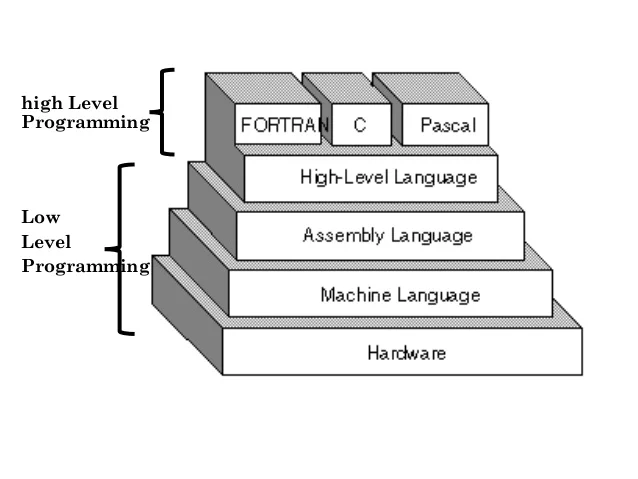
\includegraphics[width=12cm]{images/abstractionlevel_programminglangs.png}
	\caption{Abstraktionsebenen von Programmiersprachen \cite{abstractionlevels_img}}
	\label{fig:abstractionLevels}
\end{figure}
\FloatBarrier

Ein \textbf{Compiler} ist wohl das bekannteste Werkzeug zur Codegenerierung. Dieser wandelt Quellcode einer höheren Programmiersprache in Befehle einer niedrigeren Sprache um.
Ein Compiler für die Programmiersprache Java besteht aus verschiedenen Bestandteilen: Ein Scanner liest Lexeme und generiert Tokens. Der Parser generiert eine abstrakte Syntax. Im Semantik-Check wird eine getypte abstrakte Syntax generiert. Zuletzt generiert ein Code-Generator Bytecode für die JVM. Compiler sind ein fester Bestandteil von nahezu jedem Softwareentwicklungsprozess und werden aus diesem Grund der Vollständigkeit halber hier angemerkt, jedoch nicht näher behandelt.

\textbf{Modellgetriebene Softwareentwicklung (MDSD)} \textit{ist ein Oberbegriff für Techniken, die aus formalen Modellen automatisiert lauffähige Software erzeugen.} \cite[p.~11]{StahlVoelterEtAl07}

Die formalen Modelle werden meist im zugeschnittenen Modellierungssprachen wie DLS oder UML spezifiziert. Formal bedeutet in diesem Zusammenhang, dass das Modell einen bestimmten Aspekt der Software vollständig beschreibt. Dies ist essentiell für die anschließend automatische Codeerzeugung.
Ein wichtiger Begriff in diesem Kontext ist das Round-Trip Engineering. Dies beschreibt die bidirektionale Synchronisation zwischen Modellen und Quellcode. So können die Vorteile der Modellentwicklung (Übersichtlichkeit und Dokumentation) mit den der Quellcodeprogrammierung (Präzision und Spezifikation) kombiniert werden.

Die Vorteile einer modellgetriebenen Softwareentwicklung sind \cite[p.~13-16]{StahlVoelterEtAl07}:
\begin{itemize}
	\item[(a)] \textbf{Abstraktion:} Die Modelle sind einfacher und allgemeiner als der zu generierende Quellcode.
	\item[(b)] \textbf{Einheitliche Architektur:} Die Softwareerzeugung aus den Modellen erfolgt nach streng formalen Vorschriften unter Berücksichtigung eines vorgegebenen Rahmens. 
	\item[(c)] \textbf{Softwarequalität}
	Das Projekt wird durch den modellgetriebenen Entwicklungsprozess in eine einheitliche, testbare und dokumentierte Architektur gegossen. Selbstverständlich ist dies dennoch keine Garantie für gute Softwarequalität.
	\item[(d)] \textbf{Entwicklungsgeschwindigkeit:}  Durch eine höhere Softwarequalität ist das Projekt besser Wartbar und Komponenten sind besser Austauschbar, was langfristig die Entwicklungsgeschwindigkeit erhöht. Zudem gibt es immer eine Designdokumentation, was die Übersichtlichkeit erhöht.
	\item[(e)] \textbf{Interoperabilität und Plattformunabhängigkeit:} Durch die modellgetriebene Entwicklung soll eine Plattform- und Frameworkunabhängigkeit durch Standardisierung erreicht werden. Die Modelle sollen streng vom generierten Programmcode entkoppelt und somit von diesem unabhängig sein. Dies ist jedoch meist nur in der Theorie möglich und kann beispielsweise beim Round-Trip Engineering nicht gewährleistet werden.
\end{itemize}

Die Nachteile der modellgetriebenen Entwicklung sind:
\begin{itemize}
	\item[(a)] \textbf{Hoher Initialisierungsaufwand:}
	Der Initialisierungsaufwand ist sehr hoch und zahlt sich entsprechend nur bei großen Projekten aus.
	\item[(b)] \textbf{Hoher Einarbeitungsaufwand:}
	Da die modellgetriebene Entwicklung nicht so verbreitet ist wie die Verwendung herkömmlicher Programmiersprachen, jedoch eine hohe Komplexität aufweist, ist ein hoher Einarbeitungsaufwand notwendig.
\end{itemize}

Werkzeuge für die modellgetriebene Entwicklung fangen bei einfachen UML-Codegeneratoren (z.B. Visual Paradigm) an und hören bei Komplettlösungen für bestimmte Domänen (z.B. ASCET für eingebettete Automobilsoftware) auf \cite{StahlVoelterEtAl07}.

Durch AI-basierte Werkzeuge gibt es die Möglichkeit zur \textbf{Quellcodeerzeugung aus natürlicher Sprache}. Dies stellt sich vor allem für stark spezialisierte Bereiche als nützlich heraus. Ein Beispiel hierfür ist die Generierung von SQL Statements oder einfachen Programmieranweisungen aus natürlicher Sprache. 

Eine populäre Möglichkeit hierfür ist das AI-Modell OpenAI Codex. Dieses stellt auch die Basis für das Werkzeug GitHub Copilot dar, welches gemeinsam von OpenAI und GitHub entwickelt wurde \cite{openaicodex}.
Dieses Modell kann über die API oder dem Browser-Playground von OpenAI genutzt werden.
In einem Test wurde ein Ratespiel in JavaScript mittels dem OpenAI Codex Model generiert (\autoref{code:naturallangcodegen}). Aus dem in den Kommentaren angegebene Text in natürlicher Sprache wurde jeweils der darunter stehende Quellcode generiert.
\begin{lstlisting}[caption={Code aus natürlicher Sprache}, label=code:naturallangcodegen]

/* Generiere eine zufaellige Zahl zwischen 0 und 10 */
var randomNumber = Math.floor(Math.random() * 10);

/* Frage den Nutzer nach einer Texteingabe */
var userInput = prompt('Gib eine Zahl zwischen 0 und 10 ein');

/* konvertiere die Nutzereingabe in eine Zahl */
var userNumber = parseInt(userInput);

/* wenn die generierte Zufallszahl gleich der userNumber ist "gewonnen", sonst "verloren" ausgeben */
if (randomNumber === userNumber) {
	alert('gewonnen');
} else {
	alert('verloren');
}
\end{lstlisting}
\FloatBarrier
Auch die Generierung von SQL Statements liefert ein korrektes Ergebnis (\autoref{code:naturallangsql}).
\begin{lstlisting}[caption={SQL Statement aus natürlicher Sprache}, label=code:naturallangsql]
### Postgres SQL tables, with their properties:
#
# Mitarbeiter(mid, vorname, nachname)
# Teilnahme(mid, pid)
# Projekt(pid, bezeichnung)
#
### Liste die Mitarbeiternamen der Mitarbeiter des Projektes "Test" auf
---------------------------------------------------------------------
SELECT m.vorname, m.nachname
FROM Mitarbeiter m
JOIN Teilnahme t ON m.mid=t.mid
JOIN Projekt p ON t.pid=p.pid
WHERE p.bezeichnung='Test'
\end{lstlisting}
\FloatBarrier
Selbst etwas komplexere Aufgaben, wie API-Aufrufe und Deserialisierung sind möglich. Hierzu musste jedoch mit der textuellen Eingabe etwas experimentiert werden (\autoref{code:naturallangapi}) \cite{openaicodexsandbox}.
\begin{lstlisting}[caption={API Aufruf und Deserialisierung aus natürlicher Sprache}, label=code:naturallangapi]
//API aufrufen: https://jsonplaceholder.typicode.com/todos/1 
//Ergebnisse Deserialisieren & Ausgeben
//Quellcode in C#:
-------------------------------------------------------------------
using System;
using System.IO;
using System.Net;
using System.Runtime.Serialization.Json;

namespace ConsoleApp1
{
	class Program
	{
		static void Main(string[] args)
		{
			string url = @"https://jsonplaceholder.typicode.com/todos/1";
			WebRequest req = WebRequest.Create(url);
			req.Method = "GET";
			WebResponse resp = req.GetResponse();
			var json = new DataContractJsonSerializer(typeof(Todo));
			var todo = (Todo)json.ReadObject(resp.GetResponseStream());
			Console.WriteLine(todo);
		}
	}
	
	[DataContract]
	public class Todo
	{
		[DataMember]
		public bool completed { get; set; }
		[DataMember]
		public int userId { get; set; }
		[DataMember]
		public int id { get; set; }
		[DataMember]
		public string title { get; set; }
		
		public override string ToString()
		{
			return $"{completed} {id} {title}";
		}
	}
}
*/
\end{lstlisting}
\FloatBarrier
Nüchtern betrachtet bieten solche Modelle dem Entwickler jedoch kaum eine Zeitersparnis und die Ergebnisse müssten zudem stets manuell auf Korrektheit überprüft werden. Als unterstützendes Werkzeug können solche Modelle jedoch nützlich sein. Wenn der Entwickler beispielsweise nicht mit einer Programmiersprache vertraut ist, können Befehle (wie z.B. die Ein- und Ausgabe) mittels natürlicher Sprache umschrieben werden. Für die Erstellung komplexer Software sind solche Generierungsverfahren jedoch ungeeignet, da die Umschreibung mit natürlicher Sprache meist zu unscharf und inkonsistent ist \cite{DBLP:journals/corr/abs-2107-03374}. 

\textbf{Weitere Möglichkeiten}, die jedoch nur gewisse Spezialgebiete der Softwareentwicklung abdecken sind folgende \cite{Dollard2008}: Annotationen, Präprozessoranweisungen, O/R-Mapper, Interface-Definition-Languages oder Codeerzeugung durch grafischen Oberflächendesigner.

%Moderne objektorientierte Programmiersprachen wie Java und C\# bieten die %Möglichkeit Quellcode zu annotieren. Annotationen können zum einen über %Reflection zur Laufzeit ausgewertet werden und hierdurch ein bestimmtes %implementiertes Verhalten bewirken. Zum anderen gibt es bestimmte %Annotationen, die vom Compiler ausgewertet und verarbeitet werden.
\subsection{Vorteile und Grenzen}
Codegenerierung kann in der Softwareentwicklung unterschiedlich eingesetzt werden und bestimmte Vorgänge erleichtern (wie bereits in den Unterabschnitten beschrieben). Während die modellgetriebene Softwareentwicklung ein gesamtes Paradigma darstellt, sind Werkzeuge wie OpenAI Codex nur für bestimmte Randgebiete sinnvoll. Unabhängig vom verwendeten Codegenerator gilt weiterhin das bekannte Garbage In, Garbage Out Prinzip der Informatik. Darüber hinaus muss für jeden Anwendungsfall abgeschätzt werden, ob das verwendete Werkzeug einen Zeit, Qualitäts oder Produktivitätsgewinn darstellt oder eher hinderlich ist. Zu erwähnen ist außerdem, dass diese Entwicklung noch lange nicht abgeschlossen ist. Es bleibt abzuwarten was bessere Modelle und immer mehr Beispieldatensätze in Zukunft ermöglichen werden.
